\documentclass[12pt,a4paper]{report}
\usepackage[utf8]{inputenc}
\usepackage[english]{babel}
\usepackage{geometry}
\usepackage{graphicx}
\usepackage{amsmath}
\usepackage{amssymb}
\usepackage{fancyhdr}
\usepackage{hyperref}
\usepackage{titlesec}
\usepackage{tocloft}
\usepackage{setspace}
\usepackage{enumerate}
\usepackage{enumitem}
\usepackage{caption}
\usepackage{booktabs}
\usepackage{array}
\usepackage{longtable}
\usepackage{tabularx}
\usepackage{multirow}
\usepackage{float}
\usepackage{xcolor}
\usepackage{pdflscape}
\usepackage{tikz}
\usetikzlibrary{shapes.geometric,shapes.misc,arrows.meta,positioning,fit,backgrounds}

% Page geometry
\geometry{
    left=1.5in,
    right=1in,
    top=1in,
    bottom=1in
}

% Line spacing - single spacing to reduce space between lines
\singlespacing
\setlength{\parskip}{4pt}

% Base font size explicitly set to 12pt with tight baseline
\AtBeginDocument{\fontsize{12pt}{14pt}\selectfont}

% Header and footer
\pagestyle{fancy}
\fancyhf{}
\fancyhead[L]{\leftmark}
\fancyhead[R]{\thepage}
\renewcommand{\headrulewidth}{0.4pt}

% Chapter and section formatting - headings scaled relative to 12pt body text
\titleformat{\chapter}[display]
  {\normalfont\fontsize{18pt}{20pt}\selectfont\bfseries}{\chaptertitlename\ \thechapter}{12pt}{}
\titlespacing*{\chapter}{0pt}{-10pt}{20pt}

\titleformat{\section}
  {\normalfont\fontsize{15pt}{17pt}\selectfont\bfseries}{\thesection}{0.5em}{}
\titlespacing*{\section}{0pt}{10pt}{4pt}

\titleformat{\subsection}
  {\normalfont\fontsize{13pt}{15pt}\selectfont\bfseries}{\thesubsection}{0.5em}{}
\titlespacing*{\subsection}{0pt}{8pt}{3pt}

\titleformat{\subsubsection}
  {\normalfont\fontsize{12pt}{14pt}\selectfont\bfseries}{\thesubsubsection}{0.5em}{}
\titlespacing*{\subsubsection}{0pt}{6pt}{2pt}

% Hyperlink setup
\hypersetup{
    colorlinks=true,
    linkcolor=black,
    filecolor=magenta,      
    urlcolor=blue,
    citecolor=blue,
}

% Custom commands
\newcommand{\HRule}{\rule{\linewidth}{0.5mm}}

\begin{document}

% ============================================
% TITLE PAGE
% ============================================
\begin{titlepage}
\center

\vspace*{1cm}

\textsc{\LARGE \textbf{InnerVoice AI}}\\[0.5cm]
\textsc{\large Explore the emotional patterns behind text}\\[2cm]

\HRule \\[0.4cm]
{ \huge \bfseries Technical Report}\\[0.1cm]
{ \large SE - 801 - Software Project Lab III}\\[0.4cm]
\HRule \\[2cm]

\begin{minipage}{0.4\textwidth}
\begin{flushleft} \large
\textbf{Supervised by:}\\
Dr. Zerina Begum\\
Professor\\
Institute of Information Technology\\
University of Dhaka
\end{flushleft}
\end{minipage}
~
\begin{minipage}{0.4\textwidth}
\begin{flushright} \large
\textbf{Submitted by:}\\
Khandakar Mehedi Hasan\\
Institute of Information Technology\\
University of Dhaka
\end{flushright}
\end{minipage}\\[2cm]

\textbf{Submitted to:}\\
SPL 3 Program Committee\\[0.5cm]

\textbf{Submission Date:} February 26, 2026\\[0.5cm]

\includegraphics[width=0.20\textwidth]{image-1.png}\\[2cm]

\vfill


\textsc{\large Institute of Information Technology}\\
\textsc{\large University of Dhaka}\\

\end{titlepage}

% ============================================
% LETTER OF TRANSMITTAL
% ============================================
\chapter*{Letter of Transmittal}
\addcontentsline{toc}{chapter}{Letter of Transmittal}

\vspace{1cm}

\noindent 26th February, 2026

\vspace{1cm}

\noindent BSSE 4th Year Exam Committee\\
Institute of Information Technology\\
University of Dhaka

\vspace{1cm}

\noindent \textbf{Subject:} Technical Report Submission \textbf{InnerVoice AI} (Explore the emotional patterns behind text).

\vspace{1cm}

\noindent Sir,

\vspace{0.5cm}

I am submitting the technical report for our Software Project Lab 3, ``\textbf{InnerVoice AI}: Explore the emotional patterns behind text.'' This report comprehensively covers the project's technical details, including design, implementation, and testing phases. While I've tried to do my best, I welcome your feedback for improvement.

\vspace{0.5cm}

Thank you for your consideration.

\vspace{1cm}

\noindent Sincerely,

\vspace{0.5cm}

\noindent Khandakar Mehedi Hasan\\
BSSE-1326\\
Institute of Information Technology\\
University of Dhaka

\vspace{2cm}

\noindent 26.02.2026

\noindent \rule{5cm}{0.4pt}

\noindent Supervisor's Signature

% ============================================
% ACKNOWLEDGEMENT
% ============================================
\chapter*{Acknowledgement}
\addcontentsline{toc}{chapter}{Acknowledgement}

I am grateful to the Institute of Information Technology for giving me the opportunity to work on the project ``\textbf{InnerVoice AI} (Explore the emotional patterns behind text).'' I would like to convey my tremendous gratitude to my supervisor, Dr. Zerina Begum, Professor, Institute of Information Technology, University of Dhaka, for providing me with guidance and support throughout the project. Her expertise and insights were instrumental in shaping the direction of the project.

Lastly, I would like to thank my classmates. They have always been helpful and provided valuable insights from time to time.

% ============================================
% ABSTRACT
% ============================================
\chapter*{Abstract}
\addcontentsline{toc}{chapter}{Abstract}

\textbf{InnerVoice AI} is an intelligent language analysis platform designed to help users better understand how their Facebook posts reflect emotional states and personality traits. In the modern digital landscape, social media has become a primary outlet for self-expression, yet users are often unaware of how their words may appear to others or what their language reveals about their inner psychological patterns.

Leveraging advances in Natural Language Processing (NLP) and AI, \textbf{InnerVoice AI} analyzes Bangla social media text to identify sentiment, emotional tone, and personality cues. The system maps linguistic patterns to the OCEAN personality model—Openness, Conscientiousness, Extraversion, Agreeableness, and Neuroticism—providing users with meaningful, interpretable insights into their online expression.

Beyond analysis, \textbf{InnerVoice AI} promotes healthier communication by offering AI-powered rewriting suggestions when emotional imbalance, negativity, or harsh tones are detected. These suggestions help users reframe their thoughts in a more empathetic, balanced, and socially positive manner without altering the core message.

The platform also supports long-term emotional and personality tracking, allowing users to observe changes and trends over time, such as improvements in agreeableness or emotional stability. By addressing the research gap in Bangla social media text analysis, \textbf{InnerVoice AI} serves as a valuable tool for self-awareness, emotional well-being, and responsible digital communication for Bangla-speaking users.

\clearpage

% ============================================
% TABLE OF CONTENTS
% ============================================
\tableofcontents
\listoffigures
\listoftables

% ============================================
% CHAPTER 1: INTRODUCTION
% ============================================
\chapter{Introduction}

Social media, especially Facebook, has become a common place for people to share their thoughts and emotions. In Bangladesh, most of these expressions are written in Bangla and often reflect users' feelings, attitudes, and personal values. However, people are not always aware of how their posts may appear to others. What seems normal or emotional to the writer can sometimes be misunderstood as negative or aggressive.

Language often reveals emotions and personality traits without the writer realizing it. Although social media strongly affects mental well-being and public perception, tools for analyzing Bangla text are still limited. \textbf{InnerVoice AI} aims to fill this gap by analyzing Bangla Facebook posts to identify sentiment, emotional tone, and personality cues, helping users become more self-aware and communicate more positively.

\section{Purpose}

The main purpose of \textbf{InnerVoice AI} is to help users understand the emotions and personality traits reflected in their Bangla Facebook posts. The system analyzes text to identify sentiment, emotional balance, and personality patterns based on the OCEAN model. It also suggests improved rewrites when a post seems overly negative or emotionally unbalanced. Additionally, \textbf{InnerVoice AI} allows users to track changes in their emotional and personality patterns over time, supporting self-awareness and personal growth.

\section{Motivation}

\textbf{InnerVoice AI} is motivated by the strong influence of social media language on mental health and social relationships. Many users unknowingly express stress or negativity through their posts, which can cause misunderstandings. While such tools exist for English, Bangla-focused solutions are still limited. This project aims to fill that gap by providing a simple, culturally relevant tool that promotes positive communication and advances research in Bangla language analysis.

\section{Scope}

\textbf{InnerVoice AI} is designed to perform the following functions:

\begin{enumerate}
    \item Analyze Bangla Facebook posts to determine sentiment (positive, negative, or neutral).
    \item Identify underlying emotions such as joy, anger, sadness, fear, and surprise.
    \item Map linguistic patterns to personality traits based on the OCEAN model.
    \item Provide AI-assisted rewriting suggestions to promote empathetic and balanced expression.
    \item Track emotional and personality trends over time and present progress in an understandable manner.
\end{enumerate}

\section{Timeline}

Below is the proposed timeline for the \textbf{InnerVoice AI} project in a Gantt chart format:

\begin{figure}[H]
\centering
% \begin{figure}
%     \centering
%     \includegraphics[width=0.5\linewidth]{timeline.png}
%     \caption{Enter Caption}
%     \label{fig:placeholder}
% \end{figure}
\includegraphics[width=0.9\textwidth]{timeline.png}
\caption{Project Timeline - Gantt Chart}
\label{fig:timeline}
\end{figure}

\section{Purpose of Document}

The purposes of this document are:

\begin{itemize}
    \item Identify and analyze the requirements
    \item Design the architecture
    \item Design the test plan
    \item Describe methodology
    \item Reduce the development effort
    \item Improve understanding
\end{itemize}

% ============================================
% CHAPTER 2: PROJECT DESCRIPTION
% ============================================
\chapter{Project Description}

\textbf{InnerVoice AI} is designed to help people better understand how their Bangla Facebook posts reflect their emotions and personality. On social media, people often write impulsively, without thinking about how their words may sound to others. These posts can unintentionally appear negative, aggressive, or emotionally unstable. \textbf{InnerVoice AI} aims to bring awareness to this issue by analyzing written content and highlighting the emotional and psychological signals hidden within the text.

The system uses natural language processing techniques to examine Bangla posts and identify overall sentiment and specific emotions such as happiness, anger, sadness, fear, or surprise. Based on language patterns, \textbf{InnerVoice AI} also provides personality insights using the OCEAN model. When a post seems emotionally unbalanced or overly negative, the system suggests improved versions of the text that sound more calm, positive, and empathetic. Over time, users can also see how their emotional expression and personality indicators change, helping them develop healthier communication habits.

\section{Requirements}

\subsection{Normal Requirements}

Normal requirements describe the basic features that \textbf{InnerVoice AI} must have to work effectively.

\subsubsection{Functional Requirements}

\begin{itemize}
    \item \textbf{Sentiment Detection:} Analyze Bangla posts to determine whether the tone is positive, negative, or neutral.
    \item \textbf{Emotion Identification:} Detect common emotions such as joy, anger, sadness, fear, and surprise.
    \item \textbf{Personality Insight:} Provide simple personality indicators based on the OCEAN model.
    \item \textbf{Text Rewriting Support:} Suggest alternative ways to rewrite posts when strong negativity or emotional imbalance is found.
\end{itemize}

\subsubsection{Non-Functional Requirements}

\begin{itemize}
    \item \textbf{Ease of Use:} The system should be simple to use, allowing users to paste text and view results without difficulty.
    \item \textbf{Fast Response:} Analysis results should be generated within a short time.
\end{itemize}

\subsection{Expected Requirements}

Expected requirements are features users naturally assume the system will provide.

\subsubsection{Functional Requirements}

\begin{itemize}
    \item \textbf{Emotional Consistency:} Ensure that emotional analysis and personality insights make sense together.

    \item \textbf{Clear Presentation:} Show results in an easy-to-understand format, such as summaries or simple charts.
    \item \textbf{Informal Language Handling:} Correctly analyze casual Bangla, slang, and everyday expressions used on Facebook.
\end{itemize}

\subsubsection{Non-Functional Requirements}

\begin{itemize}
    \item \textbf{Reliability:} The system should work consistently without frequent errors.
\end{itemize}

\subsection{Exciting Requirements}

Exciting requirements are additional features that make the system more engaging and useful.

\subsubsection{Functional Requirements}

\begin{itemize}
    \item \textbf{Progress Tracking
:} For users who submit posts regularly, InnerVoice AI stores past results and dis-
plays changes over time, helping users notice improvements or recurring emotional
patterns.


\end{itemize}

\section{Usage Scenario for \textbf{InnerVoice AI}}

\textbf{InnerVoice AI} is a web-based platform intended for everyday users who want to understand their online behavior better.

\subsection{Access}

Users visit the \textbf{InnerVoice AI} website and either use the system directly.

\subsection{Text Submission and Analysis}

Users paste a Bangla Facebook post into the input box. The system then analyzes the text to identify sentiment, emotions, and personality-related patterns.

\subsection{Feedback and Suggestions}

After processing, \textbf{InnerVoice AI} shows:

\begin{itemize}
    \item The emotional tone of the post
    \item Detected emotions
    \item Personality indicators based on language use
\end{itemize}

If the post seems emotionally negative, the system offers rewritten versions that express the same idea in a calmer and more positive way.


\subsubsection{Example Scenario:}

A user writes a frustrated Facebook post after a stressful day. \textbf{InnerVoice AI} detects high negativity and emotional tension and suggests a softer rewrite. Over time, the user notices that their emotional balance has improved, encouraging more thoughtful online expression.

% ============================================
% CHAPTER 3: SCENARIO-BASED MODELING
% ============================================
\chapter{Scenario-Based Modeling}

Scenario-based modeling is an approach used in software development and design to create models that depict how a system behaves or reacts in various real-world situations or scenarios. These scenarios are typically based on user interactions, events, or conditions and help developers understand and visualize how the software will function in different contexts. By simulating these scenarios, developers can better identify potential issues, make informed design decisions, and ensure that the software meets user requirements across different usage contexts.

\section{Use Case Diagram}

A use case diagram is a visual representation in software engineering that illustrates how a system interacts with its external entities or actors to achieve specific goals or tasks. It shows the relationships between use cases (representing system functionalities) and actors (representing external users or systems). Use case diagrams are typically created through requirements gathering, where system functionalities and user interactions are identified and then diagrammed using specialized software modeling tools.

\subsection{Level 0 (\textbf{InnerVoice AI})}

\textbf{Primary Actor:} Facebook User

\textbf{Secondary Actor:} AI Model

\textbf{Goal in Context:} The diagram represents \textbf{InnerVoice AI}, a Bangla Facebook Post Analyzer that helps users understand and improve their social media expressions through sentiment analysis, emotion recognition, and personality insights.

\begin{figure}[H]
\centering
% \begin{figure}
%     \centering
%     \includegraphics[width=0.5\linewidth]{usercase-1.png}
%     \caption{Enter Caption}
%     \label{fig:placeholder}
% \end{figure}
\includegraphics[width=0.8\textwidth]{usercase-1.png}
\caption{Use Case Level 0 (\textbf{InnerVoice AI})}
\label{fig:usecase_level0}
\end{figure}

\subsection{Modules of Level 1 (\textbf{InnerVoice AI})}

\textbf{Primary Actor:} Facebook User

\textbf{Secondary Actor:} AI Model

\textbf{Goal in Context:} The diagram illustrates the modular architecture of \textbf{InnerVoice AI}, showing how Facebook users interact with five primary functional modules, all supported by AI models that power the analytical and generative capabilities of the system.

\begin{figure}[H]
\centering
% \begin{figure}
%     \centering
%     \includegraphics[width=0.5\linewidth]{usercase-2.png}
%     \caption{Enter Caption}
%     \label{fig:placeholder}
% \end{figure}
\includegraphics[width=0.9\textwidth]{usercase-2.png}
\caption{Use Case Level 1 (\textbf{InnerVoice AI})}
\label{fig:usecase_level1}
\end{figure}

\subsubsection{Post Analysis and Sentiment Detection}

This module is the main part of \textbf{InnerVoice AI} that analyzes user posts. Users can either paste their Bangla Facebook posts manually or upload text from their account. The system examines the text to understand the overall tone and determines whether it is positive, negative, or neutral. \textbf{InnerVoice AI} assigns a sentiment score to each post to show how strong the emotion is. It also highlights parts of the text that influence the result and explains why a certain sentiment was detected. The results are shown using simple visual tools such as sentiment indicators and highlighted words, making them easy for users to understand.

\subsubsection{Emotion Recognition}

The Emotion Recognition module goes deeper than basic sentiment analysis by identifying specific emotions expressed in a post. It detects emotions such as happiness, anger, sadness, fear, surprise, and disgust.

Each detected emotion is shown with an intensity level, helping users understand how strongly that emotion appears in their writing. The results are displayed using color-based visuals and percentage breakdowns, allowing users to see if their post contains a mix of emotions rather than just one.

\subsubsection{Personality Trait Assessment (OCEAN Model)}

This module analyzes writing patterns to provide insights into personality traits using the OCEAN model. By reviewing language style, word choices, and sentence structure, \textbf{InnerVoice AI} estimates traits such as openness, conscientiousness, extraversion, agreeableness, and neuroticism.

The system becomes more accurate as more posts are analyzed over time. Personality results are shown using simple charts and bars, allowing users to easily see which traits are more dominant and how they change with continued usage.

\subsubsection{AI Rewriting Suggestions}

When a post appears too negative, harsh, or emotionally unbalanced, this module offers rewriting suggestions. The AI generates alternative versions of the post that keep the original meaning but improve tone and clarity.

The system highlights words or phrases that may cause negative impressions and explains why suggested changes might sound more positive or empathetic. Users can compare the original and rewritten versions side by side and choose the one they prefer or modify it further.

\subsubsection{Emotional Progress Tracking}

This module helps users track their emotional and personality changes over time. \textbf{InnerVoice AI} stores analysis results from previous posts and presents them in easy-to-read graphs and summaries.

Users can see trends such as improvements in emotional balance or reductions in negative tone over weeks or months. The system also provides simple progress messages, such as increases in agreeableness or decreases in negative sentiment. This long-term tracking encourages self-awareness and supports continuous personal growth.

% ============================================
% CHAPTER 4: DATA-BASED MODELING
% ============================================
\chapter{Data-Based Modeling}

No database or data storage system is used for this tool. So this section does not contain any relevant analysis.

% ============================================
% CHAPTER 5: CLASS-BASED MODELING
% ============================================
\chapter{Class-Based Modeling}

Class-based modeling is a visual representation in software engineering that illustrates the structure of a software system using classes, their attributes, and relationships. It is commonly used in object-oriented design and modeling.

\section{Analysis Classes}

After analyzing the \textbf{InnerVoice AI} scenario, relevant nouns were identified from the problem description. These nouns were then filtered using general classification, including external entities, things, events, and system components. Further refinement was done using selection criteria, such as retained information, required services, multiple attributes, common operations, and essential system responsibilities.

The purpose of this analysis was to identify core classes that represent the internal structure of \textbf{InnerVoice AI}, which analyzes Bangla Facebook posts to extract sentiment, emotional tone, and personality traits and provide rewriting suggestions—without relying on any database system.

\subsection{Identified Key Nouns from the Scenario}

From the \textbf{InnerVoice AI} description, the following key nouns were identified as potential classes:

\begin{enumerate}
    \item User
    \item Facebook Post
    \item Sentiment
    \item Emotion
    \item Personality
    \item Rewrite Suggestion
    \item Analysis Result
    \item Text Analysis
    \item Emotional Feedback
    \item Personality Insight
\end{enumerate}

\subsection{Class Filtering and Merging}

During analysis, it was observed that several nouns represent closely related responsibilities. For example:

\begin{itemize}
    \item Sentiment, Emotion, and Personality are all analytical processes applied to text.
    \item Text Analysis acts as a coordination process rather than a standalone entity.
    \item Emotional Feedback and Personality Insights are forms of analysis output.
\end{itemize}

Based on overlapping responsibilities and to maintain a simple and modular design, similar concepts were grouped and represented through specialized analyzer classes.

\subsection{Derived Classes and Final Grouping}

After applying General Classification and Selection Criteria, the following seven analysis classes were finalized for \textbf{InnerVoice AI}:

\begin{enumerate}
    \item User
    \item Post
    \item SentimentAnalyzer
    \item EmotionAnalyzer
    \item PersonalityAnalyzer
    \item RewriteSuggestion
    \item AnalysisResult
\end{enumerate}

\section{Class Cards}

\begin{table}[H]
\centering
\caption{CRC Card (User)}
\label{tab:crc_user}
\begin{tabularx}{\textwidth}{|X|}
\hline
\textbf{User} \\
\hline
\textbf{Attributes} \\
- userId \\
- inputText \\
\hline
\textbf{Methods} \\
+ submitPost() \\
\hline
\textbf{Responsibilities} \\
$\bullet$ Submit Bangla Facebook posts for analysis \\
$\bullet$ View analysis results \\
\hline
\textbf{Collaborators} \\
$\bullet$ Post \\
\hline
\end{tabularx}
\end{table}

\begin{table}[H]
\centering
\caption{CRC Card (Post)}
\label{tab:crc_post}
\begin{tabularx}{\textwidth}{|X|}
\hline
\textbf{Post} \\
\hline
\textbf{Attributes} \\
- postId \\
- postContent \\
- language \\
\hline
\textbf{Methods} \\
- preprocessText() \\
+ sendForAnalysis() \\
\hline
\textbf{Responsibilities} \\
$\bullet$ Store the user's submitted text \\
$\bullet$ Prepare text for analysis \\
\hline
\textbf{Collaborators} \\
$\bullet$ User \\
$\bullet$ AnalysisController \\
\hline
\end{tabularx}
\end{table}

\begin{table}[H]
\centering
\caption{CRC Card (SentimentAnalyzer)}
\label{tab:crc_sentiment}
\begin{tabularx}{\textwidth}{|X|}
\hline
\textbf{SentimentAnalyzer} \\
\hline
\textbf{Attributes} \\
- sentimentLabel \\
- sentimentScore \\
\hline
\textbf{Methods} \\
+ analyzeSentiment() \\
+ calculateScore() \\
\hline
\textbf{Responsibilities} \\
$\bullet$ Determine the overall tone of the text \\
$\bullet$ Classify sentiment as positive, negative, or neutral \\
\hline
\textbf{Collaborators} \\
$\bullet$ AnalysisController \\
\hline
\end{tabularx}
\end{table}

\begin{table}[H]
\centering
\caption{CRC Card (EmotionAnalyzer)}
\label{tab:crc_emotion}
\begin{tabularx}{\textwidth}{|X|}
\hline
\textbf{EmotionAnalyzer} \\
\hline
\textbf{Attributes} \\
- detectedEmotions \\
- emotionIntensity \\
\hline
\textbf{Methods} \\
+ detectEmotion() \\
+ generateEmotionReport() \\
\hline
\textbf{Responsibilities} \\
$\bullet$ Identify emotions expressed in the text \\
$\bullet$ Measure emotional intensity \\
\hline
\textbf{Collaborators} \\
$\bullet$ AnalysisController \\
\hline
\end{tabularx}
\end{table}

\begin{table}[H]
\centering
\caption{CRC Card (PersonalityAnalyzer)}
\label{tab:crc_personality}
\begin{tabularx}{\textwidth}{|X|}
\hline
\textbf{PersonalityAnalyzer} \\
\hline
\textbf{Attributes} \\
- openness \\
- conscientiousness \\
- extraversion \\
- agreeableness \\
- neuroticism \\
\hline
\textbf{Methods} \\
+ analyzePersonality() \\
+ generatePersonalityProfile() \\
\hline
\textbf{Responsibilities} \\
$\bullet$ Analyze personality traits using the OCEAN model \\
$\bullet$ Generate a personality profile from text \\
\hline
\textbf{Collaborators} \\
$\bullet$ AnalysisController \\
\hline
\end{tabularx}
\end{table}

\begin{table}[H]
\centering
\caption{CRC Card (RewriteSuggestion)}
\label{tab:crc_rewrite}
\begin{tabularx}{\textwidth}{|X|}
\hline
\textbf{RewriteSuggestion} \\
\hline
\textbf{Attributes} \\
- originalText \\
- suggestedText \\
\hline
\textbf{Methods} \\
+ generateRewrite() \\
+ compareTexts() \\
\hline
\textbf{Responsibilities} \\
$\bullet$ Suggest an improved and emotionally balanced text \\
$\bullet$ Reduce negative or harsh expressions \\
\hline
\textbf{Collaborators} \\
$\bullet$ AnalysisController \\
$\bullet$ Post \\
\hline
\end{tabularx}
\end{table}

\begin{table}[H]
\centering
\caption{CRC Card (AnalysisController)}
\label{tab:crc_controller}
\begin{tabularx}{\textwidth}{|X|}
\hline
\textbf{AnalysisController} \\
\hline
\textbf{Attributes} \\
+ post \\
- sentimentResult \\
- emotionResult \\
- personalityResult \\
\hline
\textbf{Methods} \\
+ startAnalysis() \\
+ collectResults() \\
+ displayOutput() \\
\hline
\textbf{Responsibilities} \\
$\bullet$ Coordinate all analysis modules \\
$\bullet$ Present final results to the user \\
\hline
\textbf{Collaborators} \\
$\bullet$ Post \\
$\bullet$ SentimentAnalyzer \\
$\bullet$ EmotionAnalyzer \\
$\bullet$ PersonalityAnalyzer \\
$\bullet$ RewriteSuggestion \\
\hline
\end{tabularx}
\end{table}

\section{CRC Diagram}

The CRC diagram of the classes is given below:

\begin{figure}[H]
\centering
% \begin{figure}
%     \centering
%     
% \begin{figure}
%     \centering
%     \includegraphics[width=0.5\linewidth]{crc-2.png}
%     \caption{Enter Caption}
%     \label{fig:placeholder}
% \end{figure}
\includegraphics[width=0.9\textwidth]{crc-2.png}
\caption{CRC Diagram of \textbf{InnerVoice AI}}
\label{fig:crc_diagram}
\end{figure}

% ============================================
% CHAPTER 6: ARCHITECTURAL DESIGN
% ============================================
\chapter{Architectural Design}

Architectural design represents the high-level structure of a software system and explains how its main components are organized and interact with one another. It focuses on defining system boundaries, external entities, and communication interfaces rather than internal implementation details.

For \textbf{InnerVoice AI}, the architectural design highlights how the system processes Bangla Facebook posts to generate sentiment, emotion, personality insights, and rewriting suggestions.

\section{Architectural Context Diagram}

At the architectural design level, an Architectural Context Diagram (ACD) is used to illustrate how \textbf{InnerVoice AI} interacts with external entities beyond its system boundary. The diagram identifies external systems and actors that exchange information with the target system through defined interfaces.

External entities interacting with \textbf{InnerVoice AI} are classified as follows:

\begin{itemize}
    \item \textbf{Superordinate systems:} Systems that use InnerVoice AI as part of a higher-level workflow.
    \item \textbf{Subordinate systems:} Systems or services that InnerVoice AI depends on to perform its core functionality.
    \item \textbf{Peer-level systems:} Systems that interact with InnerVoice AI on an equal level by exchanging data.
    \item \textbf{Actors:} Individuals or devices that directly interact with the system by providing inputs or receiving outputs.
\end{itemize}

\subsection{Representation of \textbf{InnerVoice AI} in the Architectural Context Diagram}

The architectural context of \textbf{InnerVoice AI} is described below:

\begin{itemize}
    \item \textbf{Superordinate systems:} \textbf{InnerVoice AI} does not operate as a component of any higher-level system. Therefore, it has no superordinate systems.
    \item \textbf{Subordinate systems:} \textbf{InnerVoice AI} relies on Natural Language Processing (NLP) models and AI language models to analyze Bangla text. These models are used for sentiment detection, emotion recognition, personality assessment, and text rewriting. They function as subordinate systems by providing essential processing capabilities.
    \item \textbf{Peer-level systems:} \textbf{InnerVoice AI} does not directly interact with any peer-level systems. All analysis and feedback are handled within the system boundary.
    \item \textbf{Actors:} The primary actors of \textbf{InnerVoice AI} are social media users who submit Bangla Facebook posts for analysis. These users interact with the system to receive emotional insights, personality indicators, and rewriting suggestions.
\end{itemize>

\subsection{Interface Description}

Actors communicate with \textbf{InnerVoice AI} through a user interface that allows text submission and displays analysis results. Subordinate AI and NLP services interact with \textbf{InnerVoice AI} through internal processing interfaces that enable text analysis and feedback generation.

\begin{figure}[H]
\centering
% \begin{figure}
%     \centering
%     \includegraphics[width=0.5\linewidth]{arch-1.png}
%     \caption{Enter Caption}
%     \label{fig:placeholder}
% \end{figure}
\includegraphics[width=0.85\textwidth]{arch-1.png}
\caption{Architectural Context Diagram}
\label{fig:arch_context}
\end{figure}

\section{Archetypes}

The archetypes for the tool are defined below:

\begin{figure}[H]
\centering
% \begin{figure}
%     \centering
%     
% \begin{figure}
%     \centering
%     \includegraphics[width=0.5\linewidth]{arch-5.png}
%     \caption{Enter Caption}
%     \label{fig:placeholder}
% \end{figure}
\includegraphics[width=0.9\textwidth]{arch-5.png}
\caption{High-level overview of archetypes}
\label{fig:arch_highlevel}
\end{figure}

\begin{figure}[H]
\centering
% \begin{figure}
%     \centering
%     \includegraphics[width=0.5\linewidth]{arch-3.png}
%     \caption{Enter Caption}
%     \label{fig:placeholder}
% \end{figure}
% \begin{figure}
%     \centering
%     

\includegraphics[width=1\textwidth]{arch-4.png}
\caption{Archetype}
\label{fig:arch_detailed}
\end{figure}

\subsection{Text Process (Server-side)}

\textbf{SProcess User Text Using NLP:}
\begin{itemize}
    \item Receives raw text input from client-side Input Box
    \item Applies NLP libraries for text preparation
    \item Handles Bangla and English language processing
    \item Converts unstructured text into machine-readable format for analysis
\end{itemize}


\subsection{Text Analysis (Server-side)}

\textbf{Perform Text Intelligence Analysis:}
\begin{itemize}
    \item Executes Sentiment Analysis to determine emotional polarity
    \item Performs Emotion Analysis to detect feelings such as anger, happiness, sadness, etc.
    \item Applies Personality Detection models to infer user behavior pattern
    \item Uses trained AI/ML models optimized for social media text
    \item Generates structured analytical results for frontend consumption
\end{itemize}


\subsection{Rewrite (Server-side)}

\textbf{Generate Optimized Text Suggestions:}
\begin{itemize}
    \item Uses AI-based text generation models to rewrite user content
    \item Considers sentiment, emotion, and personality analysis results
    \item Adjusts tone, clarity, and positivity of the original text
    \item Produces context-aware and user-friendly rewritten text
    \item Sends best rewrite suggestions back to client-side interface
\end{itemize}

\subsection{Input Box (Client-side)}

\textbf{Capture User Text Input:}
\begin{itemize}
    \item Allows users to input Facebook posts
    \item Validates input length and format
    \item Sends text to server for processing
\end{itemize}

\subsection{Analysis Results (Client-side)}

\textbf{Display Analysis Output:}
\begin{itemize}
    \item Shows sentiment, emotion, and personality results visually
    \item Helps users understand post impact
\end{itemize}

\subsection {Rewrite Suggestion (Client-side)}

\textbf{Present AI-Generated Text:}
\begin{itemize}
    \item Displays rewritten post suggestions
    \item Enables copy and reuse functionality
\end{itemize}






\section{Top Level Components}

The overall architectural structure with top-level components is illustrated below:

\begin{figure}[H]
\centering
% \begin{figure}
%     \centering
%     
\includegraphics[width=0.9\textwidth, height=0.5\textheight]{top-1.png}

\caption{Top Level Components}
\label{fig:toplevel}
\end{figure}

\section{Mapping Requirements to Software Architecture}

The mapping of the derived components with the requirements can be shown
below:

\begin{table}[H]
\centering
\caption{Requirements to Architecture Mapping}
\label{tab:req_mapping}
\begin{tabularx}{\textwidth}{|l|X|}
\hline
\textbf{Requirement} & \textbf{Architectural Components} \\
\hline
Accept Bangla Facebook post input & User Interface, Post Component \\
\hline
Validate text input (non-empty, Bangla text) & User Interface, Post Component \\
\hline
Perform sentiment analysis & SentimentAnalyzer, NLP Service \\
\hline
Generate sentiment score and label & SentimentAnalyzer, AnalysisResult \\
\hline
Detect emotional states from text & EmotionAnalyzer, NLP Service \\
\hline
Identify emotion intensity & EmotionAnalyzer, AnalysisResult \\
\hline
Analyze personality traits using OCEAN model & PersonalityAnalyzer, NLP Service \\
\hline
Generate personality insight visualization & PersonalityAnalyzer, AnalysisResult \\
\hline
Provide AI-based rewriting suggestions & RewriteSuggestion, NLP Service \\
\hline
Preserve original meaning in rewrites & RewriteSuggestion \\
\hline


\hline
Display combined analysis results & AnalysisResult, User Interface \\
\hline
Support real-time analysis & AnalysisController, Analyzer Components \\
\hline

Allow reanalysis of modified text & Post Component, AnalysisController \\
\hline
Handle invalid input or processing errors & User Interface, AnalysisController \\
\hline
Ensure system stability during use & AnalysisController \\
% \hline
% Provide clear and user-friendly feedback & User Interface, AnalysisResult \\
\hline
\end{tabularx}
\end{table}


% ============================================
% CHAPTER 7: APPLIED METHODOLOGY
% ============================================
\chapter{Applied Methodology}

This chapter describes the internal mechanisms of \textbf{InnerVoice AI}, detailing its workflow, input handling, processing modules, and output generation.

\section{System Workflow Overview}

\textbf{InnerVoice AI} follows a structured pipeline that processes user-submitted Bangla Facebook posts through multiple analytical stages:

\begin{enumerate}
    \item User submits a Bangla Facebook post through the web interface
    \item Input validation and preprocessing
    \item Text analysis (sentiment, emotion, personality)
    \item AI-based rewriting suggestion generation
    \item Result compilation and visualization
    \item Output presentation to the user
\end{enumerate}

\section{Input Handling and Validation}

Users paste or type their Bangla Facebook posts into the text input area. Before processing, the system validates:

\begin{itemize}
    \item \textbf{Non-Empty Check:} Ensures the input contains meaningful text
    \item \textbf{Language Detection:} Verifies Bangla or English text
    \item \textbf{Length Validation:} Minimum 10 characters, maximum 5000 characters
    \item \textbf{Character Encoding:} Ensures proper UTF-8 encoding for Bangla script
\end{itemize}

\section{Text Preprocessing}

Before analysis, the input text undergoes the following preprocessing steps:

\begin{itemize}
    \item \textbf{Unicode Normalization:} Standardizes Bangla character representations
    \item \textbf{Whitespace Handling:} Removes excess spaces and normalizes line breaks
    \item \textbf{Special Character Processing:} Handles emojis and special symbols
    \item \textbf{Tokenization:} Breaks text into sentences and words, with Bangla-specific morphology handling
\end{itemize}

\section{Core Analysis Modules}

The preprocessed text is passed through three parallel analysis modules:

\begin{itemize}
    \item \textbf{Sentiment Analysis:} Determines emotional polarity using pre-trained transformer models, producing a score from $-1.0$ (negative) to $+1.0$ (positive) and classifying the post as Positive, Negative, or Neutral.
    \item \textbf{Emotion Detection:} Applies multi-label classification to detect emotions---Joy, Anger, Sadness, Fear, Surprise, and Disgust---with intensity scores for each.
    \item \textbf{Personality Trait Assessment:} Infers OCEAN personality traits (Openness, Conscientiousness, Extraversion, Agreeableness, Neuroticism) from linguistic patterns, producing normalized scores between 0 and 100.
\end{itemize}

\section{Rewriting Suggestion Generation}

When negative or emotionally imbalanced content is detected (sentiment score below $-0.3$, or high anger/sadness), the system generates rewriting suggestions using Google Gemini API. The rewritten alternatives maintain the original semantic intent while improving emotional tone. Multiple suggestions (typically 2--3) are produced and filtered for quality before being returned to the user.

\section{Result Compilation and Integration}

\subsection{Result Aggregation Architecture}

The following diagram shows how all analysis results are combined:

\begin{figure}[H]
\centering
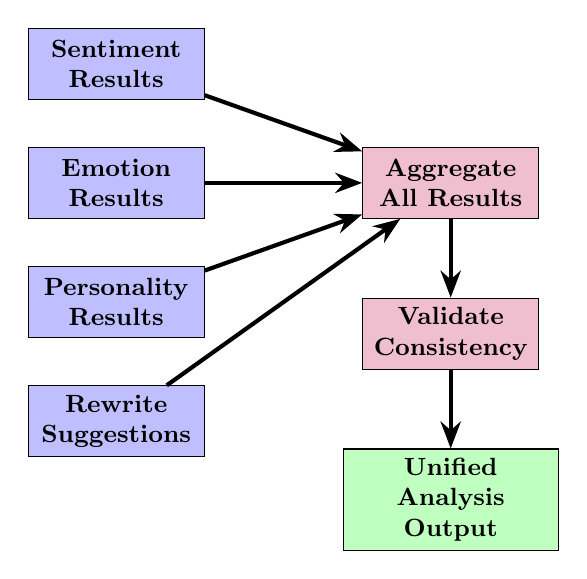
\begin{tikzpicture}[
    result/.style={rectangle, draw, fill=blue!25, text width=2cm, text centered, minimum height=0.9cm, font=\small\bfseries},
    compile/.style={rectangle, draw, fill=purple!25, text width=2cm, text centered, minimum height=0.9cm, font=\small\bfseries},
    final/.style={rectangle, draw, fill=green!25, text width=2.5cm, text centered, minimum height=0.9cm, font=\small\bfseries},
    arrow/.style={->, >=Stealth, line width=1.5pt}
]

% Input results
\node[result] (sentiment) {Sentiment\\Results};
\node[result, below=0.6cm of sentiment] (emotion) {Emotion\\Results};
\node[result, below=0.6cm of emotion] (personality) {Personality\\Results};
\node[result, below=0.6cm of personality] (rewrite) {Rewrite\\Suggestions};

% Aggregation
\node[compile, right=2cm of emotion] (aggregate) {Aggregate\\All Results};

% Validation
\node[compile, below=1cm of aggregate] (validate) {Validate\\Consistency};

% Final output
\node[final, below=1cm of validate] (final) {Unified Analysis\\Output};

% Arrows
\draw[arrow] (sentiment) -- (aggregate);
\draw[arrow] (emotion) -- (aggregate);
\draw[arrow] (personality) -- (aggregate);
\draw[arrow] (rewrite) -- (aggregate);

\draw[arrow] (aggregate) -- (validate);
\draw[arrow] (validate) -- (final);

\end{tikzpicture}
\caption{Result Compilation and Integration}
\label{fig:result_compilation}
\end{figure}

\section{Output Generation and Visualization}

The compiled results are presented to users through an intuitive interface:

\begin{itemize}
    \item \textbf{Sentiment Display:} Visual gauge showing polarity and score
    \item \textbf{Emotion Breakdown:} Bar chart of detected emotion intensities
    \item \textbf{Personality Profile:} Radar chart for OCEAN trait scores
    \item \textbf{Rewriting Suggestions:} Side-by-side comparison of original and rewritten text
\end{itemize}

\section{Technology Stack}

\begin{itemize}
    \item \textbf{Backend:} Django (Python), Django REST Framework, Hugging Face Transformers, Google Gemini API, SQLite
    \item \textbf{Frontend:} React.js, Tailwind CSS, Chart.js
    \item \textbf{NLP/ML:} NLTK, scikit-learn, pre-trained transformer models for Bangla text
\end{itemize}

% ============================================
% CHAPTER 8: TEST PLANNING
% ============================================
\chapter{Test Planning}

\section{Test Plan Overview}

\subsection{Scope}

\subsubsection{In Scope}

\begin{itemize}
    \item Language detection for Bangla (Unicode), Banglish (Roman-script), English, and mixed-language inputs
    \item Sentiment analysis (positive, negative, neutral classification)
    \item Emotion detection (joy, sadness, anger, fear, surprise, neutral)
    \item Personality trait assessment using the OCEAN model
    \item AI-powered text rewriting suggestions
    \item RESTful API endpoints (authentication, analysis, rewrite, history, progress)
    \item Data model integrity (defaults, constraints, cascade behavior, ordering)
    \item End-to-end user workflows and security controls
\end{itemize}

\subsubsection{Out of Scope}

\begin{itemize}
    \item Frontend (Chrome Extension) UI testing
    \item Load/performance and penetration testing
    \item Third-party API reliability (Google Gemini uptime)
\end{itemize}

\section{Test Strategy}

Testing follows a \textbf{V-Model} approach organized into four levels targeting distinct system layers.

\subsection{Test Levels}

\begin{table}[H]
\centering
\caption{Test Levels and Techniques}
\label{tab:test_levels}
\begin{tabularx}{\textwidth}{|l|l|X|l|}
\hline
\textbf{Level} & \textbf{Test Type} & \textbf{Scope} & \textbf{Technique} \\
\hline
1 & Unit Testing & Individual NLP/AI service modules & White-box \\
\hline
2 & Component Testing & Django ORM models and serializers & White-box \\
\hline
3 & API Integration & REST endpoint request/response contracts & Black-box \\
\hline
4 & End-to-End & Multi-step user workflows & Black-box \\
\hline
\end{tabularx}
\end{table}

\section{Test Environment}

\begin{table}[H]
\centering
\caption{Test Environment Specification}
\label{tab:test_env}
\begin{tabularx}{\textwidth}{|l|X|}
\hline
\textbf{Component} & \textbf{Specification} \\
\hline
Operating System & Ubuntu Linux 22.04 LTS \\
\hline
Runtime & Python 3.10+ \\
\hline
Framework & Django 4.x with Django REST Framework 3.x \\
\hline
Test Runner & Django \texttt{manage.py test} \\
\hline
Test Database & SQLite (in-memory, auto-created per test class) \\
\hline
Mocking Library & \texttt{unittest.mock} with \texttt{@patch} decorators \\
\hline
HTTP Client & \texttt{rest\_framework.test.APIClient} \\
\hline
\end{tabularx}
\end{table}

\section{Entry and Exit Criteria}

\subsection{Entry Criteria}

\begin{enumerate}
    \item Source code committed and all dependencies installed (\texttt{requirements.txt}).
    \item Test database schema auto-generated via Django migrations without errors.
    \item External service dependencies have corresponding mock implementations.
\end{enumerate}

\subsection{Exit Criteria}

\begin{enumerate}
    \item All planned test cases executed.
    \item All \textbf{High} priority test cases passed.
    \item No unresolved \textbf{Critical} or \textbf{High} severity defects remain.
    \item All public API endpoints and service methods covered.
\end{enumerate}

\section{Test Cases}

\subsection{Level 1: Unit Test Cases --- Service Modules}

\subsubsection{Language Detection \& Sentiment Analysis}

\begin{table}[H]
\raggedright
\caption{Test Cases --- Language Detection Service}
\label{tab:tc_lang}
\footnotesize
\begin{tabularx}{\linewidth}{|p{1.2cm}|p{2.5cm}|p{2.3cm}|p{2.8cm}|X|p{0.7cm}|}
\hline
\textbf{ID} & \textbf{Description} & \textbf{Precondition} & \textbf{Test Input} & \textbf{Expected Result} & \textbf{Type} \\
\hline
TC-LD-01 & Detect Bangla Unicode script & LanguageDetector available & \texttt{`আমি খুব খুশি আজকে'} & \texttt{language\_code = `bn'} & +ve \\
\hline
TC-LD-02 & Detect Banglish script & LanguageDetector available & \texttt{`ami khub khushi ajke'} & \texttt{language\_code = `bn'} & +ve \\
\hline
TC-LD-03 & Handle empty string & LanguageDetector available & \texttt{``} (empty) & Fallback: \texttt{`en'} & -ve \\
\hline
\end{tabularx}
\end{table}

\begin{table}[H]
\raggedright
\caption{Test Cases --- Sentiment Analysis Service}
\label{tab:tc_sent}
\footnotesize
\begin{tabularx}{\linewidth}{|p{1.2cm}|p{2.5cm}|p{2.3cm}|p{2.8cm}|X|p{0.7cm}|}
\hline
\textbf{ID} & \textbf{Description} & \textbf{Precondition} & \textbf{Test Input} & \textbf{Expected Result} & \textbf{Type} \\
\hline
TC-SA-01 & Positive sentiment & Model loaded & \texttt{`I love this amazing day!'} & \texttt{label = `positive'} & +ve \\
\hline
TC-SA-02 & Negative sentiment & Model loaded & \texttt{`I hate this terrible day'} & \texttt{label = `negative'} & +ve \\
\hline
TC-SA-03 & Bangla text sentiment & Model loaded & \texttt{`আমি খুব খুশি!'}, \texttt{lang=`bn'} & Valid label $\in$ \{positive, neutral, negative\} & +ve \\
\hline
TC-SA-04 & Fallback on model failure & \texttt{model = None} & \texttt{`Test text'} & \texttt{label=`neutral'}, \texttt{score=0.0} & -ve \\
\hline
\end{tabularx}
\end{table}

\subsubsection{Emotion Detection \& Personality Analysis}

\begin{table}[H]
\raggedright
\caption{Test Cases --- Emotion Detection Service}
\label{tab:tc_emo}
\footnotesize
\begin{tabularx}{\linewidth}{|p{1.2cm}|p{2.5cm}|p{2.3cm}|p{2.8cm}|X|p{0.7cm}|}
\hline
\textbf{ID} & \textbf{Description} & \textbf{Precondition} & \textbf{Test Input} & \textbf{Expected Result} & \textbf{Type} \\
\hline
TC-ED-01 & All emotion keys present & Detector loaded & \texttt{`I am very happy today'} & Keys  \{joy, sadness, anger, fear, surprise, neutral\} & +ve \\
\hline
TC-ED-02 & Joy dominance for positive text & Detector loaded & \texttt{`I am so happy and excited!'} & \texttt{joy > sadness} & +ve \\
\hline
TC-ED-03 & Bangla emotion detection & Detector loaded & \texttt{`আমি খুব কষ্ট পাচ্ছি'} & All six emotion keys with float values & +ve \\
\hline
\end{tabularx}
\end{table}

\begin{table}[H]
\raggedright
\caption{Test Cases --- Personality Analysis Service (OCEAN Model)}
\label{tab:tc_pers}
\footnotesize
\begin{tabularx}{\linewidth}{|p{1.2cm}|p{2.5cm}|p{2.3cm}|p{2.8cm}|X|p{0.7cm}|}
\hline
\textbf{ID} & \textbf{Description} & \textbf{Precondition} & \textbf{Test Input} & \textbf{Expected Result} & \textbf{Type} \\
\hline
TC-PA-01 & OCEAN schema validation & Analyzer instantiated & \texttt{`I love exploring new ideas'} & \texttt{traits} dict contains all 5 OCEAN keys & +ve \\
\hline
TC-PA-02 & Score range constraint & Analyzer instantiated & \texttt{`Test personality text'} &  trait: $0.0 \leq$ score $\leq 1.0$ & +ve \\
\hline
TC-PA-03 & Sentiment $\rightarrow$ Neuroticism influence & Analyzer instantiated & \texttt{sentiment=+0.9} vs \texttt{-0.9} & $N_{\text{neg}} > N_{\text{pos}}$ & +ve \\
\hline
TC-PA-04 & Null/empty input resilience & Analyzer instantiated & \texttt{None} and \texttt{``} & Default traits returned; no exception & -ve \\
\hline
\end{tabularx}
\end{table}

\subsection{Level 2 \& 3: Component and API Integration Test Cases}

\begin{table}[H]
\raggedright
\caption{Test Cases --- Django ORM Models}
\label{tab:tc_model}
\footnotesize
\begin{tabularx}{\linewidth}{|p{1.2cm}|p{2.5cm}|p{2.3cm}|p{2.8cm}|X|p{0.7cm}|}
\hline
\textbf{ID} & \textbf{Description} & \textbf{Precondition} & \textbf{Test Input} & \textbf{Expected Result} & \textbf{Type} \\
\hline
TC-MD-01 & Post default field values & Test user exists & \texttt{Post.create(text=`Hello')} & \texttt{language=`en'}, \texttt{tone=`friendly'} & +ve \\
\hline
TC-MD-02 & UUID primary key generation & Test user exists & Create Post & \texttt{post.id} is valid \texttt{uuid.UUID} & +ve \\
\hline
TC-MD-03 & User cascade deletion & Test user with 1 post & \texttt{user.delete()} & \texttt{Post.objects.count() == 0} & +ve \\
\hline
\end{tabularx}
\end{table}

\begin{table}[H]
\raggedright
\caption{Test Cases --- Authentication API (\texttt{/api/auth/})}
\label{tab:tc_auth}
\footnotesize
\begin{tabularx}{\linewidth}{|p{1.2cm}|p{2.5cm}|p{2.3cm}|p{2.8cm}|X|p{0.7cm}|}
\hline
\textbf{ID} & \textbf{Description} & \textbf{Precondition} & \textbf{Test Input} & \textbf{Expected Result} & \textbf{Type} \\
\hline
TC-AU-01 & Successful registration & No existing user & \texttt{POST} valid username, email, password & HTTP 201; response contains \texttt{token} & +ve \\
\hline
TC-AU-02 & Missing username field & None & \texttt{POST} without \texttt{username} & HTTP 400; \texttt{success=false} & -ve \\
\hline
TC-AU-03 & Duplicate username & User `existing' in DB & \texttt{POST} \texttt{username=`existing'} & HTTP 400; ``Username already exists'' & -ve \\
\hline
\end{tabularx}
\end{table}

\begin{table}[H]
\raggedright
\caption{Test Cases --- Text Analysis \& Rewrite APIs}
\label{tab:tc_analyze_rewrite}
\footnotesize
\begin{tabularx}{\linewidth}{|p{1.2cm}|p{2.5cm}|p{2.3cm}|p{2.8cm}|X|p{0.7cm}|}
\hline
\textbf{ID} & \textbf{Description} & \textbf{Precondition} & \textbf{Test Input} & \textbf{Expected Result} & \textbf{Type} \\
\hline
TC-AA-01 & Auth enforcement (analyze) & No auth token & \texttt{POST \{text: `Hello'\}} & HTTP 401 Unauthorized & -ve \\
\hline
TC-AA-02 & Empty text rejection & Authenticated user & \texttt{POST \{text: `'\}} & HTTP 400; \texttt{success=false} & -ve \\
\hline
TC-AA-03 & Bangla text analysis & Authenticated; mocked & \texttt{POST \{text: `আমি খুব খুশি!'\}} & HTTP 200; response contains \texttt{data} & +ve \\
\hline
TC-RW-01 & Auth enforcement (rewrite) & No auth token & \texttt{POST \{text: `Test'\}} & HTTP 401 & -ve \\
\hline
TC-RW-02 & Empty text rejection & Authenticated user & \texttt{POST \{text: `'\}} & HTTP 400; ``required'' & -ve \\
\hline
TC-RW-03 & Rewrite with valid \texttt{post\_id} & Post \& Analysis exist; mocked & \texttt{POST \{text, post\_id, goal\}} & HTTP 200; \texttt{success=true} & +ve \\
\hline
TC-HC-01 & Health check availability & Server running & \texttt{GET /api/health/} & HTTP 200 OK & +ve \\
\hline
TC-HC-02 & Health check public access & No auth token & \texttt{GET /api/health/} & HTTP 200 (no auth required) & +ve \\
\hline
\end{tabularx}
\end{table}

\subsection{Level 4: End-to-End Integration Test Cases}

\begin{table}[H]
\raggedright
\caption{Test Cases --- End-to-End Integration}
\label{tab:tc_e2e}
\footnotesize
\begin{tabularx}{\linewidth}{|p{1.2cm}|p{2.5cm}|p{2.3cm}|p{2.8cm}|X|p{0.7cm}|}
\hline
\textbf{ID} & \textbf{Description} & \textbf{Precondition} & \textbf{Steps} & \textbf{Expected Result} & \textbf{Type} \\
\hline
TC-IT-01 & Register $\rightarrow$ Login $\rightarrow$ Profile & Clean database & 1.~Register; 2.~Login; 3.~GET profile & All steps return success & +ve \\
\hline
TC-IT-02 & Analyze $\rightarrow$ History & Authenticated user & 1.~POST analyze; 2.~GET history & History contains 1 matching record & +ve \\
\hline
TC-IT-03 & Cross-user data isolation & Two registered users & User~A creates post; User~B queries history & User~B's history is empty & +ve \\
\hline
TC-IT-04 & Account deletion cascade & User with Post, Analysis, RewriteRecord & DELETE \texttt{/api/profile/delete/} & All related records removed from DB & +ve \\
\hline
TC-IT-05 & Token invalidation on logout & Authenticated user & 1.~GET profile; 2.~POST logout; 3.~GET profile & Step~3 returns HTTP 401 & +ve \\
\hline
\end{tabularx}
\end{table}

\section{Requirements Traceability Matrix}

\begin{longtable}{|p{0.6cm}|p{4.5cm}|p{3cm}|p{4.5cm}|}
\caption{Requirements-to-Test Traceability Matrix} \label{tab:rtm} \\
\hline
\textbf{Req.} & \textbf{Requirement Description} & \textbf{Test Case IDs} & \textbf{Coverage Status} \\
\hline
\endfirsthead
\hline
\textbf{Req.} & \textbf{Requirement Description} & \textbf{Test Case IDs} & \textbf{Coverage Status} \\
\hline
\endhead
R-01 & Detect Bangla, Banglish, and English & TC-LD-01, TC-LD-02, TC-LD-03 & \textbf{Covered} \\
\hline
R-02 & Sentiment analysis (positive, negative, neutral) & TC-SA-01 to TC-SA-04 & \textbf{Covered} \\
\hline
R-03 & Emotion detection & TC-ED-01, TC-ED-02, TC-ED-03 & \textbf{Covered} \\
\hline
R-04 & OCEAN personality trait assessment & TC-PA-01 to TC-PA-04 & \textbf{Covered} \\
\hline
R-05 & AI-based text rewriting & TC-RW-01 to TC-RW-03 & \textbf{Covered} \\
\hline
R-06 & User registration and authentication & TC-AU-01 to TC-AU-03, TC-IT-01 & \textbf{Covered} \\
\hline
R-07 & Input validation and rejection & TC-AA-01, TC-AA-02, TC-RW-02 & \textbf{Covered} \\
\hline
R-08 & Store analysis results in database & TC-MD-01 to TC-MD-03 & \textbf{Covered} \\
\hline
R-09 & User data isolation & TC-IT-03 & \textbf{Covered} \\
\hline
R-10 & Account deletion with cascade & TC-IT-04, TC-MD-03 & \textbf{Covered} \\
\hline
R-11 & Token-based session management & TC-IT-05, TC-AU-01 & \textbf{Covered} \\
\hline
R-12 & System availability (health check) & TC-HC-01, TC-HC-02 & \textbf{Covered} \\
\hline
\end{longtable}

\section{Test Execution Summary}

\begin{table}[H]
\centering
\caption{Test Execution Summary by Category}
\label{tab:test_exec_summary}
\begin{tabularx}{\textwidth}{|X|c|c|c|c|}
\hline
\textbf{Test Category} & \textbf{Test File} & \textbf{Total} & \textbf{Passed} & \textbf{Status} \\
\hline
Language Detection (Unit) & \texttt{test\_services\_language.py} & 3 & 3 & \textcolor{green!60!black}{\textbf{PASS}} \\
\hline
Sentiment Analysis (Unit) & \texttt{test\_services\_sentiment.py} & 4 & 4 & \textcolor{green!60!black}{\textbf{PASS}} \\
\hline
Emotion Detection (Unit) & \texttt{test\_services\_emotion.py} & 3 & 3 & \textcolor{green!60!black}{\textbf{PASS}} \\
\hline
Personality Analysis (Unit) & \texttt{test\_services\_personality.py} & 4 & 4 & \textcolor{green!60!black}{\textbf{PASS}} \\
\hline
Text Analysis API & \texttt{test\_analysis\_views.py} & 3 & 3 & \textcolor{green!60!black}{\textbf{PASS}} \\
\hline
Rewrite API & \texttt{test\_rewrite\_views.py} & 3 & 3 & \textcolor{green!60!black}{\textbf{PASS}} \\
\hline
Authentication API & \texttt{test\_auth\_views.py} & 3 & 3 & \textcolor{green!60!black}{\textbf{PASS}} \\
\hline
Data Models (Component) & \texttt{test\_models.py} & 3 & 3 & \textcolor{green!60!black}{\textbf{PASS}} \\
\hline
End-to-End Integration & \texttt{test\_integration.py} & 5 & 5 & \textcolor{green!60!black}{\textbf{PASS}} \\
\hline
Health Check & \texttt{test\_health.py} & 2 & 2 & \textcolor{green!60!black}{\textbf{PASS}} \\
\hline
\textbf{Total} & & \textbf{33} & \textbf{33} & \textcolor{green!60!black}{\textbf{ALL PASS}} \\
\hline
\end{tabularx}
\end{table}

\section{Defect Summary and Risk Assessment}

\subsection{Defect Summary}

No critical or high-severity defects remained unresolved at the conclusion of testing. The language detector's Banglish heuristic may classify some English words as Banglish by design, to minimize false negatives for Bangla-speaking users.

\subsection{Risk Assessment}

\begin{table}[H]
\centering
\caption{Testing Risk Assessment}
\label{tab:risk_assessment}
\begin{tabularx}{\textwidth}{|l|X|l|X|}
\hline
\textbf{Risk ID} & \textbf{Risk Description} & \textbf{Severity} & \textbf{Mitigation} \\
\hline
RSK-01 & External API (Gemini) unavailability & High & Mocked in tests; fallback responses implemented \\
\hline
RSK-02 & Inaccurate results for novel Bangla slang & Medium & Banglish dictionary regularly updated \\
\hline
RSK-03 & Database migration failures in production & Low & In-memory SQLite used; migrations tested separately \\
\hline
\end{tabularx}
\end{table}

\section{Conclusion}

All 33 test cases across four test levels have been executed and passed. Every functional requirement is covered by at least one test case, confirming input validation, authentication enforcement, data isolation, cascade integrity, and graceful degradation.

% ============================================
% CHAPTER 9: USER MANUAL AND USER INTERFACE
% ============================================
\chapter{User Manual and User Interface}

\section{System Overview}

\textbf{InnerVoice AI} is a web-based application with an optional Chrome Extension that analyzes Bangla (and Banglish) social media posts to extract emotional insights, personality traits, and communication patterns. The system is built using a modern client--server architecture:

\begin{itemize}
    \item \textbf{Frontend (Web Application):} A React.js single-page application built with Vite, styled using Tailwind CSS and shadcn/ui components. The web interface provides pages for text analysis, rewriting, history review, progress tracking, and user settings. It communicates with the backend via RESTful API calls.
    
    \item \textbf{Frontend (Chrome Extension):} A Manifest V3 Chrome Extension that provides a compact popup interface for quick text analysis and history viewing directly from the browser toolbar, without navigating to the full web application.
    
    \item \textbf{Backend (Django REST API):} A Python-based Django REST Framework server that handles user authentication (token-based), text analysis pipelines (sentiment, emotion, personality), AI-powered text rewriting via Google Gemini, progress tracking, behavioral analytics, and data persistence using SQLite.
    
    \item \textbf{NLP \& AI Services:} A suite of modular Python services including \texttt{SentimentAnalyzer}, \texttt{EmotionDetector}, \texttt{PersonalityAnalyzer}, \texttt{LanguageDetector}, \texttt{BanglaProcessor}, \texttt{ContextAnalyzer}, \texttt{TextRewriter}, \texttt{ProgressTracker}, and \texttt{BehavioralAnalytics}---all orchestrated to deliver comprehensive text analysis.
\end{itemize}

The system supports three language modes: pure Bangla (Unicode), Banglish (Bangla written in English script), and English---automatically detecting the language and applying appropriate analysis pipelines.

\section{User Manual}

% ---- 9.2.1 Registration ----
\subsection{Step 1: User Registration}

To begin using \textbf{InnerVoice AI}, new users must create an account.

\begin{enumerate}
    \item Navigate to the \textbf{InnerVoice AI} website.
    \item Click on the \textbf{``Register''} link on the login page.
    \item Fill in the registration form with the following fields:
    \begin{itemize}
        \item \textbf{Username:} A unique username for the account.
        \item \textbf{Email:} A valid email address.
        \item \textbf{Password:} Must be at least 8 characters, containing lowercase, uppercase, and a number.
        \item \textbf{Confirm Password:} Re-enter the password for verification.
    \end{itemize}
    \item A real-time password strength indicator shows which criteria are met.
    \item Click the \textbf{``Create Account''} button to complete registration.
\end{enumerate}

\begin{figure}[H]
\centering
\includegraphics[width=0.85\textwidth]{module-2.png}
\caption{Fig: Registration Page -- showing the sign-up form with username, email, password fields, password strength indicators, and the ``Create Account'' button.}
\label{fig:ui_register}
\end{figure}

% ---- 9.2.2 Login ----
\subsection{Step 2: User Login}

Returning users can log in to access their account and analysis history.

\begin{enumerate}
    \item Navigate to the \textbf{InnerVoice AI} login page.
    \item Enter the registered \textbf{username} and \textbf{password}.
    \item Click the \textbf{``Sign In''} button.
    \item Upon successful login, the user is redirected to the \textbf{Dashboard}.
\end{enumerate}


\begin{figure}[H]
\centering
\includegraphics[width=0.85\textwidth]{module-1.png}
\caption{Fig: Login Page -- showing the login form with username and password fields, the ``Sign In'' button, and the link to the registration page.}
\label{fig:ui_login}
\end{figure}


% ---- 9.2.3 Dashboard ----
\subsection{Step 3: Exploring the Dashboard}

After logging in, users are taken to the \textbf{Dashboard}, which provides an overview of their activity and analysis statistics.

\begin{enumerate}
    \item The Dashboard displays:
    \begin{itemize}
        \item \textbf{Summary statistics:} Total analyses performed, emotional streak, and recent activity.
        \item \textbf{Sentiment trend chart:} A line/area chart showing how sentiment scores have changed over recent analyses.
        \item \textbf{Emotion distribution:} A visual breakdown of detected emotions across all analyzed posts.
        \item \textbf{OCEAN personality radar:} A radar chart showing aggregated personality trait scores.
        \item \textbf{Quick action buttons:} Links to navigate to Analyze, Rewrite, History, and Progress pages.
    \end{itemize}
    \item Users can refresh data or navigate to detailed pages from the Dashboard.
\end{enumerate}

% \begin{figure}[H]
% \centering
% \fbox{\parbox{0.85\textwidth}{\vspace{6cm}\centering\textit{[Insert Screenshot Here]}\vspace{0.5cm}}}
% \caption{Fig: Dashboard Page (Top Section) -- showing summary statistics cards, welcome message, and quick action buttons.}
% \label{fig:ui_dashboard_top}
% \end{figure}

\begin{figure}[H]
\centering
\includegraphics[width=0.85\textwidth]{module-4.png}
\caption{Fig: Dashboard Page (Top Section) – showing summary statistics
cards, welcome message, and quick action buttons.
}
\label{fig:ui_dashboard-top}
\end{figure}


\begin{figure}[H]
\centering
\includegraphics[width=0.85\textwidth]{module-5.png}
\caption{Fig: Dashboard Page (Charts Section) -- showing the sentiment trend area chart, emotion distribution bar chart, and OCEAN personality radar chart.
}
\label{fig:ui_dashboard-top}
\end{figure}

% ---- 9.2.4 Text Analysis ----
\subsection{Step 4: Analyzing Text}

The core functionality of \textbf{InnerVoice AI} is text analysis.

\begin{enumerate}
    \item Navigate to the \textbf{``Analyze''} page from the sidebar or Dashboard.
    \item Paste or type a Bangla/Banglish/English text into the text area.
    \item Click the \textbf{``Analyze''} button.
    \item The system processes the text and displays:
    \begin{itemize}
        \item \textbf{Sentiment Score:} A numerical score indicating positive, negative, or neutral tone with a visual gauge.
        \item \textbf{Detected Emotions:} A list of emotions (e.g., joy, anger, sadness, fear, surprise) with confidence percentages.
        \item \textbf{OCEAN Personality Traits:} Scores for Openness, Conscientiousness, Extraversion, Agreeableness, and Neuroticism.
        \item \textbf{Language Detection:} Whether the text was detected as Bangla, Banglish, or English.
        \item \textbf{Flagged Words:} Words or phrases identified as strongly negative or emotionally charged.
    \end{itemize}
    \item If negative tone is detected, a \textbf{``Rewrite''} button appears to navigate to the Rewrite page.
\end{enumerate}

\begin{figure}[H]
\centering
\includegraphics[width=0.85\textwidth]{module-6.png}
\caption{Fig: Text Analysis Page (Input Section) -- showing the text input area with a sample Bangla post and the ``Analyze'' button.
}
\label{fig:ui_text_analysis-input}
\end{figure}

\begin{figure}[H]
\centering
\includegraphics[width=0.85\textwidth]{module-7.png}
\caption{Fig: Text Analysis Page (Results Section) – showing sentiment score
gauge, detected emotions with percentages, OCEAN personality radar chart, and
Flagged Words.
}
\label{fig:ui_text_analysis-result}
\end{figure}

% ---- 9.2.5 Text Rewriting ----
\subsection{Step 5: Rewriting Text}

When a post contains negative or harsh language, users can use the AI-powered rewriting feature.

\begin{enumerate}
    \item After analysis, click the \textbf{``Rewrite''} button, or navigate to the \textbf{``Rewrite''} page from the sidebar.
    \item The original text is pre-filled (if coming from the Analyze page), or the user can paste new text.
    \item Flagged words from the original text are highlighted for reference.
    \item Select a \textbf{rewriting goal} (e.g., more positive, more empathetic, more professional, calmer tone).
    \item Click the \textbf{``Rewrite''} button.
    \item The system generates an AI-powered rewritten version of the text that preserves the original meaning while improving the emotional tone.
    \item Users can \textbf{copy} the rewritten text to use on social media.
\end{enumerate}



\begin{figure}[H]
\centering
\includegraphics[width=0.85\textwidth]{module-8.png}
\caption{Fig: Rewrite Page – showing the original text with highlighted flagged
words, rewriting goal selection options, and the "Rewrite" button.
}
\label{fig:ui_text_rewrite}
\end{figure}


% ---- 9.2.6 Analysis History ----
\subsection{Step 6: Viewing Analysis History}

Users can review their previously analyzed posts.

\begin{enumerate}
    \item Navigate to the \textbf{``History''} page from the sidebar.
    \item The page displays a \textbf{master--detail layout}:
    \begin{itemize}
        \item \textbf{Left panel:} A scrollable list of past analyses showing text snippets, sentiment badges, emotion icons, and timestamps.
        \item \textbf{Right panel:} A detailed analysis report for the selected item.
    \end{itemize}
    \item Users can \textbf{search} through history by text content.
    \item Users can \textbf{filter} history by sentiment type (positive, negative, neutral).
    \item Users can \textbf{sort} history by newest or oldest first.
    \item Pagination is provided for navigating large histories.
    \item Clicking any history item opens its full analysis report in the right panel.
\end{enumerate}

\begin{figure}[H]
\centering
\includegraphics[width=0.85\textwidth]{module-9.png}
\caption{Fig: History Page -- showing the master-detail layout with a list of past analyses on the left (with search, filter, and sort controls) and a detailed analysis report panel on the right.}
\label{fig:ui_text_history}
\end{figure}

% ---- 9.2.7 Progress Tracking ----
\subsection{Step 7: Tracking Emotional Progress}

Users who analyze posts regularly can track their emotional and personality trends over time.

\begin{enumerate}
    \item Navigate to the \textbf{``Progress''} page from the sidebar.
    \item The page displays:
    \begin{itemize}
        \item \textbf{Sentiment trend over time:} A line chart showing how overall sentiment has changed across analyses.
        \item \textbf{Emotion frequency breakdown:} Charts showing which emotions appear most often.
        \item \textbf{OCEAN personality evolution:} A radar chart showing how personality trait scores have shifted over time.
        \item \textbf{Behavioral analytics:} Insights such as posting frequency, language usage patterns, emotional streaks, and communication style analysis.
        \item \textbf{Activity heatmap:} Visual representation of analysis activity across different time periods.
    \end{itemize}
    \item Users can select different time ranges (e.g., last 7 days, last 30 days, all time) to view trends.
\end{enumerate}

\begin{figure}[H]
\centering
\includegraphics[width=0.85\textwidth]{module-10.png}
\caption{Fig: Progress Page (Sentiment \& Emotion Trends) -- showing sentiment trend line chart and emotion frequency charts with time range selector.}
\label{fig:ui_text_history}
\end{figure}


% ---- 9.2.8 Settings ----
\subsection{Step 8: Managing Settings}

Users can customize their account and application preferences.

\begin{enumerate}
    \item Navigate to the \textbf{``Settings''} page from the sidebar.
    \item The Settings page has multiple sections:
    \begin{itemize}
        \item \textbf{Profile:} Update display name, email, and upload a profile avatar.
        \item \textbf{Appearance:} Switch between Light, Dark, and System themes.
        \item \textbf{Notifications:} Configure notification preferences.
        \item \textbf{Security:} Change password.
        \item \textbf{Data \& Privacy:} Export all personal data as JSON or delete the account entirely.
    \end{itemize}
\end{enumerate}

\begin{figure}[H]
\centering
\includegraphics[width=0.85\textwidth]{module-11.png}
\caption{Fig: Settings Page -- showing profile update, appearance (theme), security (password change), and data \& privacy (export/delete) sections.}
\label{fig:ui_settings}
\end{figure}


% ---- 9.2.9 Chrome Extension ----
\subsection{Step 9: Using the Chrome Extension}

\textbf{InnerVoice AI} also offers a Chrome Extension for quick analysis directly from the browser.

\begin{enumerate}
    \item Install the \textbf{InnerVoice AI} Chrome Extension from the browser.
    \item Click the extension icon in the browser toolbar to open the popup.
    \item The extension provides two tabs:
    \begin{itemize}
        \item \textbf{Analyze Tab:} Paste or type text for quick sentiment, emotion, and personality analysis.
        \item \textbf{History Tab:} View recent analysis history.
    \end{itemize}
    \item Results are displayed in a compact format optimized for the extension popup (400$\times$600 px).
\end{enumerate}

\begin{figure}[H]
\centering
\includegraphics[width=0.85\textwidth]{module-12.png}
\caption{Fig: Chrome Extension popup -- showing the Analyze tab for quick text input and the History tab for recent results.}
\label{fig:chrome-extension}
\end{figure}

\section{Challenges Addressed by InnerVoiceAI}

\textbf{InnerVoice AI} addresses several key challenges in Bangla social media text analysis:

\textbf{Lack of Bangla NLP Tools.} English NLP tools are widely available, but tools for Bangla social media text are extremely limited. InnerVoice AI fills this gap with purpose-built sentiment, emotion, and personality analysis for Bangla.

\textbf{Banglish Processing.} A large portion of Bangla social media content uses Banglish (Bangla written in Roman script), with no standard romanization scheme. A dedicated \texttt{BanglaProcessor} handles transliteration and normalization using a Banglish dictionary and heuristic rules.

\textbf{Context-Dependent Sentiment.} Bangla negation, sarcasm, and informal slang make simple keyword-based analysis unreliable. The \texttt{ContextAnalyzer} handles negation patterns, intensifiers, and contextual meaning to produce accurate sentiment scores.

\textbf{Promoting Self-Awareness and Positive Communication.} Many users are unaware of the emotional tone their posts project. InnerVoice AI provides immediate feedback, tracks emotional patterns over time, and offers AI-powered rewriting suggestions to help users communicate more constructively online.

\section{Access Frontend and Backend Code}

The complete source code for \textbf{InnerVoice AI} is hosted on GitHub and can be accessed as follows:

\subsection{GitHub Repository}

The full project source code is available at:

\begin{center}
\textbf{Repository:} \url{https://github.com/Rizon1326/InnerVoiceAI}
\end{center}

\subsection{Backend Setup}

To set up and run the backend server locally:

\begin{enumerate}
    \item \textbf{Clone the repository:}
    \begin{verbatim}
    git clone https://github.com/Rizon1326/InnerVoiceAI.git
    cd InnerVoiceAI/backend
    \end{verbatim}
    
    \item \textbf{Create and activate a virtual environment:}
    \begin{verbatim}
    python -m venv venv
    source venv/bin/activate    # Linux/macOS
    venv\Scripts\activate       # Windows
    \end{verbatim}
    
    \item \textbf{Install dependencies:}
    \begin{verbatim}
    pip install -r requirements.txt
    \end{verbatim}
    
    \item \textbf{Apply database migrations:}
    \begin{verbatim}
    python manage.py migrate
    \end{verbatim}
    
    \item \textbf{Run the development server:}
    \begin{verbatim}
    python manage.py runserver
    \end{verbatim}
    
    The backend API will be available at \texttt{http://localhost:8000/api/}.
\end{enumerate}

\subsection{Frontend Setup (Web Application)}

To set up and run the frontend web application locally:

\begin{enumerate}
    \item \textbf{Navigate to the frontend directory:}
    \begin{verbatim}
    cd InnerVoiceAI/frontend
    \end{verbatim}
    
    \item \textbf{Install Node.js dependencies:}
    \begin{verbatim}
    npm install
    \end{verbatim}
    
    \item \textbf{Start the development server:}
    \begin{verbatim}
    npm run dev
    \end{verbatim}
    
    The web application will be available at \texttt{http://localhost:5173/}.
\end{enumerate}

\subsection{Frontend Setup (Chrome Extension)}

To build and load the Chrome Extension:

\begin{enumerate}
    \item \textbf{Build the extension:}
    \begin{verbatim}
    cd InnerVoiceAI/frontend
    npm run build:ext
    \end{verbatim}
    
    \item \textbf{Load in Chrome:}
    \begin{itemize}
        \item Open \texttt{chrome://extensions/} in Google Chrome.
        \item Enable \textbf{Developer mode} (toggle in the top-right corner).
        \item Click \textbf{``Load unpacked''} and select the \texttt{dist-extension/} folder.
    \end{itemize}
    
    \item The InnerVoice AI icon will appear in the browser toolbar.
\end{enumerate}

\subsection{Running Tests}

To run the backend test suite:

\begin{verbatim}
    cd InnerVoiceAI/backend
    python -m pytest tests/ -v --tb=short
\end{verbatim}

This executes all 33 test cases covering unit, component, API integration, and end-to-end tests as described in Chapter~8 (Test Planning).

\subsection{API Endpoints Reference}

The backend exposes the following RESTful API endpoints:

\begin{table}[H]
\centering
\caption{InnerVoice AI API Endpoints}
\label{tab:api_endpoints}
\small
\begin{tabularx}{\textwidth}{|l|l|X|}
\hline
\textbf{Method} & \textbf{Endpoint} & \textbf{Description} \\
\hline
GET & \texttt{/api/health/} & Health check (public) \\
\hline
POST & \texttt{/api/auth/register/} & User registration \\
\hline
POST & \texttt{/api/auth/login/} & User login (returns token) \\
\hline
POST & \texttt{/api/auth/logout/} & User logout (invalidates token) \\
\hline
POST & \texttt{/api/analyze/} & Analyze text for sentiment, emotion, personality \\
\hline
POST & \texttt{/api/rewrite/} & AI-powered text rewriting \\
\hline
GET & \texttt{/api/history/} & Retrieve analysis history \\
\hline
GET & \texttt{/api/progress/} & Get user progress data \\
\hline
GET & \texttt{/api/progress/trends/} & Get emotional trends \\
\hline
GET & \texttt{/api/progress/behavioral-analytics/} & Get behavioral analytics \\
\hline
GET & \texttt{/api/metrics/} & Get user metrics \\
\hline
GET & \texttt{/api/profile/} & Get user profile \\
\hline
POST & \texttt{/api/profile/avatar/} & Upload profile avatar \\
\hline
GET & \texttt{/api/profile/export/} & Export all user data as JSON \\
\hline
DELETE & \texttt{/api/profile/delete/} & Delete user account \\
\hline
GET & \texttt{/api/statistics/} & Public project statistics \\
\hline
\end{tabularx}
\end{table}

All endpoints except \texttt{/api/health/}, \texttt{/api/auth/register/}, \texttt{/api/auth/login/}, and \texttt{/api/statistics/} require token-based authentication via the \texttt{Authorization: Token <token>} header.

% ============================================
% CHAPTER 10: CONCLUSION
% ============================================
\chapter{Conclusion}

\textbf{InnerVoice AI} bridges the gap in Bangla social media text analysis, offering users practical insights into their emotional expression and personality patterns. By combining sentiment analysis, emotion recognition, and OCEAN-based personality assessment, the system transforms passive reading into active self-awareness.

The platform goes beyond mere analysis—it promotes healthier digital communication. When negative or harsh tones are detected, AI-powered rewriting suggestions help users express themselves more positively while preserving their intended message. This encourages thoughtful expression and emotional intelligence in online spaces.

The modular architecture ensures reliability, scalability, and future growth. Each component operates independently yet contributes to a unified experience. Comprehensive testing validates accuracy and usability, making \textbf{InnerVoice AI} a dependable tool for self-reflection.

Ultimately, \textbf{InnerVoice AI} empowers Bangla-speaking users to understand their digital footprint, improve communication quality, and foster emotional well-being. It represents a meaningful step toward building a more empathetic and self-aware online community.

% ============================================
% BIBLIOGRAPHY (Optional)
% ============================================
% \begin{thebibliography}{99}
% \bibitem{ref1}
% Author Name. \textit{Book Title}. Publisher, Year.
% \end{thebibliography}

\end{document}
